\documentclass[12pt,onepage,onecolumn]{article}
\usepackage{master}

\newcommand{\orden}[1]{\scriptsize\ttfamily #1\normalsize}
\author{Félix J. Marcelo Wirnitzer}
\title{Instalación de Arch Linux}
\date{}

\begin{document}
  \maketitle
  \section{Descargamos la ISO de Arch Linux}
\begin{frame}
\begin{enumerate}
    \item<1-> Comprobamos si la ISO tiene más de un mes. Si es así, hay que descargar la última. Siempre se publica una nueva cada
        primero de mes.
\item <2-> Hay que descargarla de \small{\verb+https://ftp.tu-chemnitz.de/pub/linux/archlinux/iso/archlinux-2026.03.01-x86\_64.iso+}

\item <3> Y tostamos\dots
\end{enumerate}
\end{frame}

  \section{Establecemos el teclado en español}

  \begin{center}
    \begin{tcolorbox}[title=Establecemos el teclado en español]
      \orden{loadkeys es}
    \end{tcolorbox}
   \end{center}

  \newpage
\section{Comprobamos qué tipo de arranque tiene la placa}

\begin{center}
\vspace{5mm}
 
 
 \begin{tcolorbox}[title=Comprobamos qué tipo de arranque tiene la placa]
    \orden{ls /sys/firmware/efi/efivars}
 \end{tcolorbox}
 
 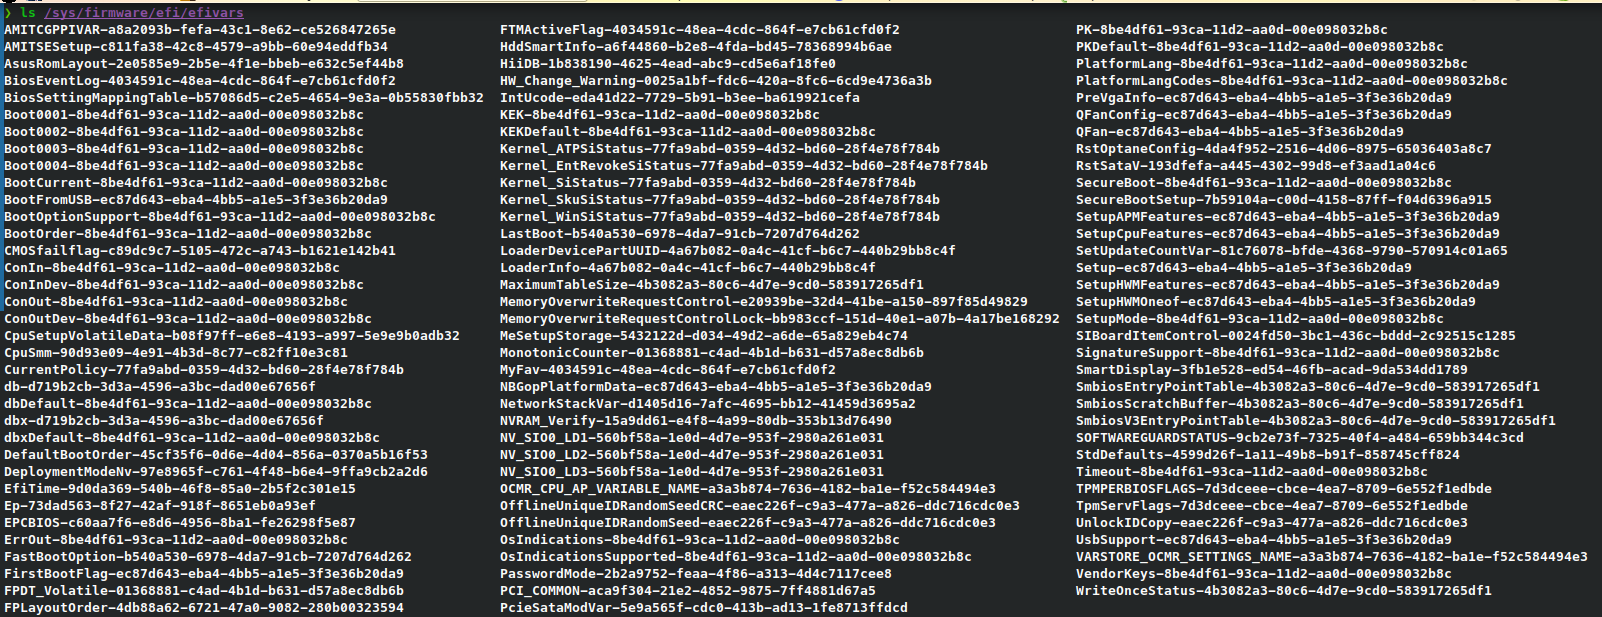
\includegraphics[width=.95\textwidth]{3 UEFI.png}\\
\end{center}

 \vspace{15mm}

 \begin{tcolorbox}[title=Si  vemos  esta  salida\,  entonces  es  un  arranque  \btrojo{UEFI}]
Instalaremos el paquete \tazul{grub} y, adicionalmente, \tazul{efibootmgr}.
 \end{tcolorbox}

 \vspace{15mm}

 \begin{tcolorbox}[title=Si  no la vemos entonces  es  un arranque  \brojo{BIOS}]
Instalaremos únicamente el paquete \tazul{grub}.
 \end{tcolorbox}
 \newpage

  \section{¿Tenemos conexión a Internet?}

\begin{center}
    
  \begin{tcolorbox}[title=Comprobamos la conexión a Internet]
	\orden{\ttfamily ping -c 4 google.es}
  \scriptsize
  \begin{verbatim}
  PING google.es (172.217.17.3) 56(84) bytes de datos.
  64 bytes desde mad07s09-in-f3.1e100.net (172.217.17.3): icmp_seq=1 ttl=119 tiempo=63.4 ms
  64 bytes desde mad07s09-in-f3.1e100.net (172.217.17.3): icmp_seq=2 ttl=119 tiempo=77.9 ms
  64 bytes desde mad07s09-in-f3.1e100.net (172.217.17.3): icmp_seq=3 ttl=119 tiempo=34.3 ms
  64 bytes desde mad07s09-in-f3.1e100.net (172.217.17.3): icmp_seq=4 ttl=119 tiempo=33.3 ms

  --- google.es estadísticas ping ---
  4 paquetes transmitidos, 4 recibidos, 0\% packet loss, time 3004ms
  rtt min/avg/max/mdev = 33.302/52.228/77.929/19.152 ms
  \end{verbatim}
	\end{tcolorbox}

	\begin{tcolorbox}[title=Nota]
		En caso de que sea un portátil o un ordenador con conexión inalámbrica, se deberá usar la aplicación {\color{blue}\ttfamily iwctl}.\\

  \textbf{Pasos a seguir}\\
  Para conectarse a la red WiFi, debemos saber el nombre de nuestro dispositivo primero, para esto un ip link y ya estamos del otro lado. Para los comandos a continuación usaremos \tazul{wlan0} como nombre de dispositivo y supongamos además que nuestra SSID es \tmarron{redCasa} con clave \trojo{1234567890}.

\begin{center}
  \verb+iwctl --passphrase 1234567890 station wlan1 connect redCasa+
\end{center}

Si todo va bien debería funcionar la orden \tmarron{ping}
	\end{tcolorbox}
\end{center}
\newpage

  \section{Para proceder al particionado}
\begin{frame}

\begin{center}
\color{blue}Para proceder al particionado\vspace{10mm}\color{black}

\only<1>{\begin{tcolorbox}[title=Si se trata de un disco duro mecánido o una unidad SSD]
	\orden{cfdisk /dev/sda}
\end{tcolorbox}}


\only<2>{\begin{tcolorbox}[title=Pero si se trata de una unidad M.2]
	\orden{cfdisk /dev/nvme0n1}
\end{tcolorbox}}



\end{center}
\end{frame}

\subsection{Consideraciones}
\begin{frame}
	\begin{center}
		\begin{tcolorbox}[title=Hay que tener en cuenta si el disco está particionado como \textbf{MBR} o como \textbf{GPT}]	
		
			\begin{tabular}{ccc}
				&  \textbf{MBR} & \textbf{GPT} \\
				\textbf{Partición BIOS}	& No hace falta & Sí, en formato FAT32\\
				\textbf{Partición UEFI}	& No hace falta & Sí, en formato FAT32\\
			\end{tabular}	
		\end{tcolorbox}
		
	\end{center}
\end{frame}

\subsection{Ejemplo de particionado MBR}
\begin{frame}
	\begin{center}
	
	
	\begin{tcolorbox}[title=Ejemplo de particionado MBR]	
		\begin{ttfamily}
			\begin{tabular}{llll}
			{\color{blue}/dev/sda1} &  {\color{red}/} 	  & {\color{brown}ext4} & \color{orange}mkfs.ext4 /dev/sda1\color{blue} \\
			{\color{blue}/dev/sda2} &  {\color{red}swap}  & {\color{brown}swap} & \color{orange}mkswap /dev/sda2\color{blue} \\
			{\color{blue}/dev/sda3} &  {\color{red}/home} & {\color{brown}ext4} & \color{orange}mkfs.ext4 /dev/sda3\color{blue} \\
		\end{tabular}
		\end{ttfamily}
	\end{tcolorbox}
	
	Aquí no importa si el arranque es de tipo BIOS o UEFI.
	\end{center}
\end{frame}

\subsection{Ejemplo de particionado GPT}
\begin{frame}
	\begin{center}
		
		\begin{tcolorbox}[title=Ejemplo de particionado GPT con BIOS]
		\begin{ttfamily}
			\begin{tabular}{llll}
				{\color{blue}/dev/sda1} &  {\color{red}BIOS}  & {\color{brown}fat32} & {\color{orange}mkfs.fat -F32 /dev/sda1}\\
				{\color{blue}/dev/sda2} &  {\color{red}/} 	  & {\color{brown}ext4}  & {\color{orange}mkfs.ext4 /dev/sda1} \\
				{\color{blue}/dev/sda3} &  {\color{red}swap}  & {\color{brown}swap}  & {\color{orange}mkswap /dev/sda2} \\
				{\color{blue}/dev/sda4} &  {\color{red}/home} & {\color{brown}ext4}  & {\color{orange}mkfs.ext4 /dev/sda3}
			\end{tabular}
		\end{ttfamily}
		\end{tcolorbox}
		
	Es recomendable que la partición BIOS sea el primero de todos.
	\end{center}
	
\end{frame}

\subsection{Ejemplo de particionado GPT}
\begin{frame}
\begin{center}
	
	\begin{tcolorbox}[title=Ejemplo de particionado GPT con EFI]
		\begin{ttfamily}
			\begin{tabular}{llll}
				{\color{blue}/dev/sda1} &  {\color{red}EFI}  & {\color{brown}fat32} & {\color{orange}mkfs.fat -F32 /dev/sda1}\\
				{\color{blue}/dev/sda2} &  {\color{red}/} 	  & {\color{brown}ext4}  & {\color{orange}mkfs.ext4 /dev/sda1} \\
				{\color{blue}/dev/sda3} &  {\color{red}swap}  & {\color{brown}swap}  & {\color{orange}mkswap /dev/sda2} \\
				{\color{blue}/dev/sda4} &  {\color{red}/home} & {\color{brown}ext4}  & {\color{orange}mkfs.ext4 /dev/sda3}
			\end{tabular}
		\end{ttfamily}
	\end{tcolorbox}
	
	Es recomendable que la partición EFI sea el primero de todos.
\end{center}
\end{frame}

\subsection{Montaje de las particiones}
\begin{frame}
\begin{center}
	
	\begin{tcolorbox}[title=Sabiendo que {\ttfamily /dev/sda2} será la partición raíz:]
		\begin{ttfamily}
			\orden{mount /dev/sda2 /mnt}
		\end{ttfamily}
	\end{tcolorbox}\pause
	
	
	\begin{tcolorbox}[title=Si es una instalación en un disco GPT con una partición BIOS o UEFI habrá que hacer,colframe=alert,colback=white]
		\orden{mount --mkdir /dev/sda1 /mnt/boot}
	\end{tcolorbox}
	
\end{center}
\end{frame}

\subsection{Montaje de las particiones}
\begin{frame}
	\begin{center}
		\begin{tcolorbox}[title=Montamos la partición \textit{swap}]
			\orden{swapon /dev/sda3}
			\tcblower
			La partición \textit{home} se montará más adelante.
		\end{tcolorbox}\pause
	\end{center}
\end{frame}

  \section{Instalación del sistema base}
\subsection{Actualización del catálogo de paquetes}
\begin{frame}
\begin{tcolorbox}[title=Primero actualizamos el catálogo de paquetes]
    \orden{pacman -Sy}
\end{tcolorbox}
\end{frame}

\subsection{Instalación}
\begin{frame}
	
\only<1>{\begin{tcolorbox}[title=Instalación con BIOS: {\color{red}\ttfamily grub-bios}]
		\begin{ttfamily}
		\scriptsize
		\begin{tabular}{l}
			pacstrap -K /mnt base base-devel linux linux-firmware sudo ntfs-3g networkmanager curl aria2 zsh neovim \textbackslash  \\
			\hspace{21mm} {\color{red}grub-bios} sddm plasma openssh git
		\end{tabular}
		\normalsize
		\end{ttfamily}
\end{tcolorbox}}
		
\pause
	
\only<2>{\begin{tcolorbox}[title=Instalación con UEFI: {\color{red}\ttfamily grub} y {\color{red}\ttfamily efibootmgr}]
		\begin{ttfamily}
		\scriptsize
		\begin{tabular}{l}
			pacstrap -K /mnt base base-devel linux linux-firmware sudo ntfs-3g networkmanager curl aria2 zsh neovim \textbackslash  \\
			\hspace{21mm} {\color{red}grub efibootmgr} sddm plasma openssh git
		\end{tabular}
		\normalsize
		\end{ttfamily}
  \end{tcolorbox}}

\end{frame}

\subsection{Paquetes instalados}
\begin{frame}
  \begin{tcolorbox}[title=Explicación de los paquetes instalados]

  \scriptsize
  \begin{description}
    \item[base:] Conjunto mínimo de paquetes para definir una instalación básica de Arch Linux.
    \item[base-devel:] Conjunto de paquetes necesarios para crear software a partir del código fuente.
    \item[linux:] El propio \textit{kernel}.
    \item[linux-firmware:] Controladores para hardware común.
    \item[sudo:]  Quieres ejecutar comandos como root, ¿verdad?
    \item[ntfs-3g:]  Controlador del sistema de archivos NTFS y utilidades necesarias para trabajar con unidades NTFS.
    \item[networkmanager:] Facilita detección y configuración para que los sistemas se conecten automáticamente a las redes.
    \item[curl:] Herramienta de línea de comandos y una biblioteca para transferir datos mediante URL.
    \item[aria2:] aria2 es una ligera utilidad de descarga multiprotocolo y multifuente.
    \item[zsh:] \textit{Shell} potente que funciona como shell interactivo y como intérprete de lenguajes de scripting.
    \item[neovim:] Editor de texto plano de gran potencia.
    \item[grub:] Gestor multiarranque.
    \item[openssh:] Protocolo de red para iniciar una sesión en una máquina remota.
    \item[git:] Programa para control de versiones.
  \end{description}
\end{tcolorbox}
	
\end{frame}



  \section{Generación del fichero fstab}

% Nota: las particiones ya deben estar montadas desde la sección de particionado.
% Si se ha seguido el paso anterior, /home ya está montado en /mnt/home.

\subsection{Generación de {\ttfamily fstab}}

\begin{tcolorbox}[title=Generación de fstab]
    \begin{lstlisting}[style=bashstyle]
genfstab -U /mnt >> /mnt/etc/fstab
    \end{lstlisting}
\end{tcolorbox}
    
\begin{tcolorbox}[title=Comprobamos que se ha generado correctamente]
    \begin{lstlisting}[style=bashstyle]
cat /mnt/etc/fstab
    \end{lstlisting}
\end{tcolorbox}

\subsection{Entrada a la raíz}

  \begin{tcolorbox}[title=Y entramos en la partición {\ttfamily /mnt}]
    \begin{lstlisting}[style=bashstyle]
arch-chroot /mnt
    \end{lstlisting}
  \end{tcolorbox}
\newpage

  \section{Configuración de Arch Linux}
\subsection{Zona horaria}
\begin{frame}

  \begin{tcolorbox}[title=Establecemos la zona horaria que es {\color{red}Atlántico/Canarias}]
    \orden{ln -sf /usr/share/zoneinfo/{\color{red}Atlantic/Canary} /etc/localtime}
\end{tcolorbox}\pause

\begin{tcolorbox}[title=A continuación ejecutamos]
    \orden{hwclock --systohc}
\end{tcolorbox}
\end{frame}

  \section{Configuración de Arch Linux}
\subsection{Localización}
\begin{frame}

    {\color{blue}Editamos con {\ttfamily nano} {\color{red}\ttfamily /etc/locale.gen}}\\\vspace{3mm}

    \visible<1->{\begin{tcolorbox}[title=Aquí configuramos el idioma]
      \orden{nano /etc/locale.gen}
    \end{tcolorbox}}
    \visible<2->{\begin{tcolorbox}[title=Descomentamos la línea que contenga {\color{red}es\_ES.UTF-8 UTF-8}]
      \centering
      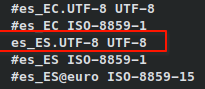
\includegraphics[width=30mm]{9 localizacion.png}\\
    \end{tcolorbox}}\pause
    
    \visible<3>{\begin{tcolorbox}[title=Y tras guardar:]
      \orden{locale-gen}
    \end{tcolorbox}}
    
\end{frame}

\begin{frame}
    \begin{tcolorbox}[title=Para establecer el idioma por defecto:]
	    \orden{echo 'LANG=es\_ES.UTF-8' > /etc/locale.conf}\\
    	\orden{echo 'KEYMAP=es' > /etc/vconsole.conf}
    \end{tcolorbox}
\end{frame}


%   \section{Configuración de Arch Linux}
\subsection{Red}
\begin{frame}
    \begin{tcolorbox}[title=Le damos nombre a nuestro ordenador]
      \orden{echo Lusitania > /etc/hostname}
    \end{tcolorbox}
\end{frame}

\subsection{Red}
\begin{frame}

    \begin{tcolorbox}[title=Añadimos las siguientes líneas en {\ttfamily /etc/hosts}]
    \begin{ttfamily}
    \begin{tabular}{ll}
    	127.0.0.1    &  localhost \\
	    ::1          &  localhost \\
	    127.0.1.1    &  Lusitania
    \end{tabular}
    \end{ttfamily}
  \end{tcolorbox}
    
\end{frame}

\begin{frame}
\begin{tcolorbox}[title=Habilitamos {\ttfamily NetworkManager} para su arranque automático]
	\orden{systemctl enable NetworkManager}
\end{tcolorbox}
\end{frame}



%   \section{Usuarios}

\subsection{Establecemos la contraseña de \textit{root}}
\begin{frame}
\begin{tcolorbox}[title=Establecemos la contraseña del usuario \textit{root}]
    \orden{passwd}
\end{tcolorbox}
\end{frame}


\subsection{Nuevo usuario \textit{non-root}}
\begin{frame}
    Seguiremos los siguientes pasos para la creación de nuestro usuario {\color{red}\textbf{viriato}} con su contraseña {\color{red}\textbf{iberia}}.
      \begin{tcolorbox}[title=Creamos el grupo de \textbf{viriato}.]
       	\orden{groupadd {\color{red}viriato}}
      \end{tcolorbox}\pause
   	
    \begin{tcolorbox}[title=Creamos el usuario.]
   	\orden{useradd {\color{blue}viriato} {\color{brown}-m} {\color{red}-g viriato}}
    \tcblower
    \scriptsize
   	Con el parámetro {\color{brown}\textbf{-m}} indicamos que debe crear el directorio {\ttfamily\color{red}/home/viriato} y {\color{green}\textbf{-g}} para indicar el grupo principal del usuario.
    \end{tcolorbox}\pause
   	
    \begin{tcolorbox}[title=Le ponemos al usuario una contraseña.]
     \orden{passwd {\color{blue}viriato}}
    \end{tcolorbox}
\end{frame}

 \subsection{Privilegios \textit{sudo} para \color{blue}viriato}
\begin{frame}
		Queremos darle a {\color{brown}viriato} privilegios de tipo \textit{sudo}.

    \begin{tcolorbox}[title=Para ellos debemos editar el fichero {\ttfamily\color{red}/etc/sudoers}]
		\orden{nano /etc/sudoers}
    \end{tcolorbox}
		
		
   \begin{tcolorbox}[title=Y añadimos la siguiente línea]
   	 \orden{viriato ALL=(ALL:ALL) NOPASSWD:ALL}
     \tcblower
     \scriptsize
 	   Guardamos y cerramos el fichero.
   \end{tcolorbox}
		
\end{frame}

%   \section{Instalación del paquete de microcode ($\mu$cod e)}
\begin{frame}


  En Arch Linux, las actualizaciones de microcódigo están disponibles a través de paquetes oficiales que todo usuario debería instalar en sus sistemas.\\\vspace{5mm}
    
Los fabricantes de procesadores como Intel y AMD lanzan a menudo actualizaciones de estabilidad y seguridad para el procesador. Estas actualizaciones son cruciales para la estabilidad del sistema.\\\vspace{5mm}
    
\only<1>{\begin{tcolorbox}[title=En el caso de Intel]\orden{pacman -S intel-ucode}\end{tcolorbox}} 
\only<2>{\begin{tcolorbox}[title=En el caso de AMD]\orden{pacman -S amd-ucode}\end{tcolorbox}} 
\end{frame}

%   \section{Cargador de arranque}
\subsection{GRUB}
\begin{frame}

    Configuramos GRUB, el cargador de arranque. Debemos tener en cuenta si la placa tiene BIOS o UEFI como vimos al principio.
    
    \only<1>{\begin{tcolorbox}[title=Si se trata de un arranque BIOS con disco mecánico o una unidad SSD]%
        \orden{grub-install /dev/sda}%
    \end{tcolorbox}}
    \only<2>{\begin{tcolorbox}[title=Si se trata de un arranque BIOS con una unidad M.2]%
        \orden{grub-install /dev/nvme0n1}%
    \end{tcolorbox}\vspace{5mm}}
    \only<3>{\begin{tcolorbox}[title=Si se trata de un arranque UEFI]
      \orden{grub-install --target=x86\_64-efi --efi-directory=/boot --bootloader-id=grub}
    \end{tcolorbox}\vspace{5mm}}

    \only<4>{\begin{tcolorbox}[title=Guardamos la configuración:]
      \orden{grub-mkconfig -o /boot/grub/grub.cfg}
      \tcblower
      \scriptsize
      Y si no muestra un mensaje de error, podemos reiniciar comprobando que podemos arrancar Arch Linux.
    \end{tcolorbox}}\pause\vspace{5mm}
     
    
\end{frame}

%   \section{Repositorio AUR}
\subsection{Introducción}
\begin{frame}
	El \textbf{Arch User Repository (AUR)} es un repositorio comunitario para usuarios de Arch.\\\vspace{10mm}\pause
	
	Contiene descripciones de paquetes (PKGBUILDs) que permiten compilar un paquete desde el código fuente con makepkg y luego instalarlo mediante {\color{brown}\texttt{pacman}}.\\\vspace{10mm}\pause
	
  El \textbf{AUR} se creó para organizar y compartir nuevos paquetes de la comunidad y para ayudar a acelerar la inclusión de paquetes populares en el repositorio extra.\\\vspace{10mm}\pause
	
	La aplicación que usaremos para instalar paquetes de los repositorios de \textbf{AUR} será {\color{brown}\texttt{yay}}.
		
\end{frame}

%   \section{Instalación de {\color{brown}\texttt{yay}}}
\subsection{Proceso de instalación}
\begin{frame}
	\begin{center}
		{\color{blue}Pasos a seguir:}\vspace{3mm}
		
      \begin{tcolorbox}[title=Descargamos los ficheros desde \textbf{Github}:]

			\orden{git clone https://aur.archlinux.org/yay.git}
      \end{tcolorbox}\pause
			
      \begin{tcolorbox}[title=Ahora vamos al directorio y compilamos:]
			\orden{cd yay}\vspace{1mm}
      
			\orden{makepkg -si}
      \end{tcolorbox}\pause
			
		\visible<4->{Para instalar software solo hay que escribir {\color{red}\texttt{yay}} en lugar de {\color{red}\texttt{pacman}} sin necesidad de usar la orden {\color{red}\texttt{sudo}}}.\\\visible<5>{Desde este momento podemos instalar todos los paquetes con {\color{red}\texttt{yay}}.}
		\end{center}
\end{frame}

%   \section{Entornos gráficos}

Antes de instalar un escritorio hay que asegurarse de que los drivers de vídeo
están correctamente instalados. Es uno de los puntos donde más alumnos se atascan.

\subsection{Identificar la tarjeta gráfica}

\begin{tcolorbox}[title=Identificamos el hardware gráfico]
\begin{lstlisting}[style=bashstyle]
lspci | grep -i vga
\end{lstlisting}
\end{tcolorbox}

\subsection{Drivers de vídeo}

\begin{tcolorbox}[title=Intel o AMD — Mesa (recomendado)]
\begin{lstlisting}[style=bashstyle]
yay -S mesa
\end{lstlisting}
\tcblower
\scriptsize Proporciona soporte OpenGL y Vulkan para Intel y AMD. Opción por defecto y recomendada para Wayland.
\end{tcolorbox}

\begin{tcolorbox}[title=NVIDIA — driver propietario]
\begin{lstlisting}[style=bashstyle]
yay -S nvidia nvidia-utils
\end{lstlisting}
\tcblower
\scriptsize Para RTX 2000 o más nuevas puede usarse también \texttt{nvidia-open}. Para kernels LTS, usa \texttt{nvidia-lts}.
\end{tcolorbox}

\begin{tcolorbox}[title=Hardware antiguo o genérico]
\begin{lstlisting}[style=bashstyle]
yay -S xf86-video-vesa
\end{lstlisting}
\end{tcolorbox}

\subsection{Entornos de escritorio}

\begin{tcolorbox}[title=Instalar \textbf{GNOME}]
\begin{lstlisting}[style=bashstyle]
yay -S gnome gdm
systemctl enable gdm
\end{lstlisting}
\tcblower
\scriptsize Entorno completo con excelente soporte Wayland. \texttt{gdm} es su display manager nativo.
\end{tcolorbox}

\begin{tcolorbox}[title=Instalar \textbf{KDE Plasma}]
\begin{lstlisting}[style=bashstyle]
yay -S plasma sddm
systemctl enable sddm
\end{lstlisting}
\tcblower
\scriptsize Altamente configurable. \texttt{sddm} es el display manager recomendado por KDE.
\end{tcolorbox}

\begin{tcolorbox}[title=Instalar \textbf{XFCE} (opción ligera)]
\begin{lstlisting}[style=bashstyle]
yay -S xfce4 xfce4-goodies lightdm lightdm-gtk-greeter
systemctl enable lightdm
\end{lstlisting}
\tcblower
\scriptsize Ideal para hardware con pocos recursos. Consume sensiblemente menos RAM que GNOME o KDE.
\end{tcolorbox}

\subsection{Compositores Wayland (caso avanzado)}

\begin{tcolorbox}[title=\textbf{Hyprland} — tiling compositor Wayland]
\begin{lstlisting}[style=bashstyle]
yay -S hyprland waybar wofi kitty
\end{lstlisting}
\tcblower
\scriptsize Se inicia desde la TTY con \texttt{Hyprland}. Sin necesidad de display manager.
\end{tcolorbox}

\begin{tcolorbox}[title=\textbf{Sway} — equivalente Wayland de i3]
\begin{lstlisting}[style=bashstyle]
yay -S sway swaybar dmenu foot
\end{lstlisting}
\tcblower
\scriptsize Se inicia con \texttt{sway}. Más estable y conservador que Hyprland.
\end{tcolorbox}

\subsection{Reinicio y verificación}

\begin{tcolorbox}[title=Salimos del chroot y reiniciamos]
\begin{lstlisting}[style=bashstyle]
exit
umount -R /mnt
reboot
\end{lstlisting}
\tcblower
\scriptsize Al arrancar deberías ver la pantalla de login del display manager.
Si el sistema arranca en TTY, comprueba: \texttt{systemctl status gdm} (o \texttt{sddm}, \texttt{lightdm}).
\end{tcolorbox}

%   \section{Últimas consideraciones}
\subsection{Fin}

    Con esto podemos dar por terminada la instalación de Arch Linux.\vspace{5mm}

    \begin{tcolorbox}[title=En caso de dudas siempre se puede consultar su wiki en español]
      \url{https://wiki.archlinux.org/title/Main_page_(Español)}
    \end{tcolorbox}

%   % ============================================================
%  Portada elegante — Instalación de Arch Linux
%  Usa: xcolor, tikz (via tcolorbox[most]), graphicx, fontspec
% ============================================================

\definecolor{archblue}{HTML}{1793D1}
\definecolor{coverdark}{HTML}{16213E}
\definecolor{covermid}{HTML}{0F3460}

\newgeometry{margin=0pt}
\thispagestyle{empty}
\pagecolor{coverdark}

\begin{tikzpicture}[remember picture, overlay]

  %% ── Fondo: degradado simulado con rectángulos ──────────────
  \fill[covermid]
    (current page.south west) rectangle (current page.north east);
  \fill[coverdark, opacity=0.6]
    ([yshift=8cm]current page.south west) rectangle (current page.north east);

  %% ── Franja izquierda ───────────────────────────────────────
  \fill[archblue]
    (current page.south west)
    rectangle ([xshift=6pt]current page.north west);

  %% ── Franja inferior ────────────────────────────────────────
  \fill[archblue!80!black]
    (current page.south west)
    rectangle ([yshift=2.4cm]current page.south east);

  %% ── Círculos decorativos tras el logo ──────────────────────
  \node[circle, fill=archblue!8!coverdark,  minimum size=10.5cm]
    at ([yshift=-8cm]current page.north) {};
  \node[circle, draw=archblue!30, line width=0.8pt, minimum size=10.9cm]
    at ([yshift=-8cm]current page.north) {};
  \node[circle, draw=archblue!12, line width=0.4pt, minimum size=12cm]
    at ([yshift=-8cm]current page.north) {};

  %% ── Logo Arch Linux ────────────────────────────────────────
  \node at ([yshift=-8cm]current page.north) {%
    
\includegraphics[width=6cm]{arch_linux.png}%
  };

  %% ── Título principal ───────────────────────────────────────
  \node[
    text=white!80!coverdark,
    font=\fontsize{32}{40}\selectfont\bfseries
  ] at ([yshift=-14.8cm]current page.north) {Instalación de};

  \node[
    text=archblue,
    font=\fontsize{54}{64}\selectfont\bfseries
  ] at ([yshift=-17.8cm]current page.north) {Arch Linux};

  %% ── Línea decorativa ───────────────────────────────────────
  \draw[archblue!50, line width=0.6pt]
    ([yshift=-19.8cm, xshift=-5.5cm]current page.north)
    -- ([yshift=-19.8cm, xshift=5.5cm]current page.north);

  %% ── Subtítulo ──────────────────────────────────────────────
  \node[
    text=white!50!coverdark,
    font=\large\itshape
  ] at ([yshift=-21.2cm]current page.north)
    {Guía de instalación paso a paso};

  %% ── Autor y período en franja inferior ─────────────────────
  \node[text=white, font=\normalsize\bfseries]
    at ([yshift=1.4cm]current page.south)
    {Félix J. Marcelo Wirnitzer};

  \node[text=white!70!black, font=\small]
    at ([yshift=0.7cm]current page.south)
    {Curso \periodo};

\end{tikzpicture}

\null\vfill
\newpage
\restoregeometry
\pagecolor{white}
\color{black}

\end{document}
